%% This LaTeX-file was created by Marco Kienzle (Marco.Kienzle@gmail.com)
%% 
%% Do not edit this file unless you know what you are doing.

% This latex template was created to produce document that will be transformed into MS Word document.
% The command to do so is 
% latex article.tex
% bibtex article
% latex2rtf -Z3 -P /usr/local/share/latex2rtf/cfg/:/tmp/latex2rtf-1.9.16a/scripts/ article.tex

\documentclass{article}
%\documentclass{nrc2}
%\journal{cjfas}

\usepackage[dvips]{color}

%\usepackage{bbding}
\usepackage{natbib}
\usepackage{setspace}
\usepackage{amsmath}
\usepackage{graphicx}
%\usepackage{psfig}
\usepackage{verbatim}
\usepackage{rotating}
\usepackage{multirow}
\usepackage{longtable}
\usepackage{booktabs}
\usepackage{subfigure}
\usepackage{lineno}
\usepackage{url}
\renewcommand{\baselinestretch}{1.5} % set space between lines to 1.5

\setlength{\oddsidemargin}{0.5cm}
\setlength{\evensidemargin}{0.5cm}
\setlength{\textwidth}{17cm}
%\setlength{\textheight}{23cm}
%\addtolength{\oddsidemargin}{-3cm}
%\addtolength{\evensidemargin}{-3cm}

\usepackage{fancyhdr}
\pagestyle{fancyplain} %Note the \fancyplain command !!!
%\renewcommand{\chaptermark}[1]{\markboth{#1}{}}
%\renewcommand{\sectionmark}[1]{\markright{#1}{}}
\lhead[\fancyplain{E}{EE}] {\fancyplain{}{}}
\chead[\fancyhead{}{}]{\fancyplain{}{—Draft—}}
\cfoot [ ] {\copyright \hspace{0.1cm} The State of Queensland (through the Department of Agriculture, Fisheries and Forestry Queensland) [2015] \begin{center} \thepage \end{center}}

\begin{document}

\linenumbers

\title{hazard function models to estimate fish mortality rates by maximum likelihood from age data, with application to the sea mullet ({\it mugil cephalus}) fishery on the east-coast of Australia}

%\author{Marco Kienzle\footnote{Queensland Dept of Agriculture, Fisheries and Forestry, Ecosciences Precinct, Joe Baker St, Dutton Park, Brisbane, QLD 4102, Australia; \newline University of Queensland, School of Agriculture and Food Sciences, St. Lucia, QLD 4072, Australia}, Jason McGilvray\footnote{Queensland Dept of Agriculture, Fisheries and Forestry, Ecosciences Precinct, Joe Baker St, Dutton Park, Brisbane, QLD 4102, Australia} and You-Gan Wang\footnote{University of Queensland, Centre for Applications in Natural Resource Mathematics, School of Mathematics and Physics, St. Lucia, QLD 4072, Australia}}
\author{Marco Kienzle\footnote{Queensland Dept of Agriculture, Fisheries and Forestry, Ecosciences Precinct, Joe Baker St, Dutton Park, Brisbane, QLD 4102, Australia; \newline University of Queensland, School of Agriculture and Food Sciences, St. Lucia, QLD 4072, Australia}}

\maketitle

\abstract{Fisheries management agencies around the world collect age data for the purpose of assessing the status of natural resources in their juridiction. Estimates of mortality rates are central to assess the sustainability of fish stocks exploitation. Survival analysis has seldom been applied to fisheries research despite its widespread use in medical research and engineering to estimate failure rates. In this paper, we present a variety of hazard functions to model the dynamic of a fishery and estimate by maximum likelihood all parameters necessary for a stock assessment (including natural and fishing mortality rates as well as gear selectivity) from a sample of fish age. These methods were tested by Monte Carlo simulations to assert that they provide un-biased estimates of these quantities. An application to the Queensland's sea mullet fishery (Australia) dataset provided an estimate of natural mortality equal to 0.319 $\pm$ 0.165 year$^{-1}$.


%% Survival analysis has seldomed be used in this area of research despite estimate fish mortality ratesSurvival analysis was applied to fisheries catch at age data to develop maximum likelihood estimators for stock assessment. This new method estimated natural mortality, fishing mortality and catchability from typical catch at age matrices. Monte Carlo simulations suggested estimates were unbiased and provided a better fit than the traditional multinomial approach. 

%% Application to a dataset from Queensland's sea mullet fishery (Australia) estimated natural mortality to be equal to 0.319 $\pm$ 0.165 year$^{-1}$.
}

\section{Introduction} One of the purposes of stock assessment is to estimate mortalities affecting fish stocks. This task is much easier for species that can be aged compared to, for example crustaceans, which aging is not possible. The reason lies in that mortality and longevity are inversely related hence age is a measure, albeit inverse, of mortality. The central mortality model used in fisheries research was proposed by Baranov to describe the variation of the number of fish belonging to a cohort through time \citep{quin99b}. This deterministic exponential model has a statistical counterpart in the form of the exponential probability distribution function which first and second moments quantify the relationship between longevity (age) and mortality rate \citep{cow98b}. Adopting a statistical view of this problem allowed to develop maximum likelihood estimators \citep{Burnb03} of parameters of importance to stock assessment scientists. The branch of statistics focused on survival analysis has created and refined methods to estimate mortality rates \citep{cox84b} which are widely applied in the fields of medical research and engineering. \\ 

%The present article describes an application of survival analysis to fisheries catch at age data.
Despite the commonalities between survival analysis for medical and fisheries research, this theory has seldom been applied to animal ecology \citep{Pollock1989}: to our knowledge, there hasn't been any application to fish age data for the purpose of stock assessment. In this manuscript, we described how to apply survival analysis to create likelihood functions of catch at age for the purpose of estimating natural and fishing mortalities as well as gear selectivity. We started with a simplistic example of constant natural and fishing mortality to introduce fundamental concepts from survival analysis before moving to more sophisticated cases leading to its application to real data from the sea mullet fishery in Queensland (Australia). The proposed methods were tested with simulated data to characterize some of their properties and their capacity to estimate population dynamic parameters of interest. Finally, the application to the mullet fishery case study provided specific estimates of natural mortality, catchability and selectivity. \\


\section{Materials and methods} 

Fish aging is possible thanks to a little bone called the otolith which is present in their ears. An otolith accumulate materials and increases in size throughout the entire lifespan of a fish. Microscopic analyses of sections of an otolith shows a series of marks, similar to tree rings, that can be used to assign each individual to a specific age-group.\\

Most fisheries institute around the world have a sampling program dedicated to collect a representative sample of fish each year to determine the distribution of age of any species of interest. In most cases, the data are binned into age-groups of width 1 year. For this reason, we split the lifespan of cohorts from their birth ($t \in [0;\infty]$) into $n$ yearly intervals from $a_{1}=0$ to the maximum age of $a_{n+1}$ years. While the theory presented in this document used that particular subdivision of time ($t$), un-equal ones also applies. In fact, an un-equal subdivision of time was used for the sea mullet case study.
 


\subsection{The likelihood for constant natural and fishing mortality rates} 
           The exponential decrease in abundance of individuals belonging to a single cohort due to constant natural ($M$) and fishing ($F$) mortality rates was described from a survival analysis point of view \citep{scimar42,cox84b} using a constant hazard function of time ($t$) and parameters $\theta$

\begin{equation}
h(t; \theta) = M + F
\end{equation}

The probability density function (pdf) describing survival from natural and fishing mortality is

\begin{equation}
f(t; \theta) = (M + F) \ e^{-(M+F)t} = \underbrace{M \times e^{-(M+F)t}}_{=f_{1}(t; \theta)} + \underbrace{F \times e^{-(M+F)t}}_{=f_{2}(t; \theta)}
\end{equation}

Since age data belonging to individuals dying from natural causes are generally not available to fisheries scientists, we used only the component of the pdf that relates to fishing mortality ($f_{2}(t; \theta)$). This component of $f(t; \theta)$ integrates over the entire range of $t$ to 

\begin{align}
 \int_{t=0}^{t=\infty} f_{2}(t; \theta) \ dt &= \int_{t=0}^{t=\infty} F \times e^{-(M+F)t} \ dt\\
                                         &= \int_{t=0}^{t=\infty} f(t; \theta) \ dt - \int_{t=0}^{t=\infty} M \times e^{-(M+F)t} \ dt\\
                                         &= 1 - \int_{t=0}^{t=\infty} M \times e^{-(M+F)t} \ dt \\
                                         &= 1 - \frac{M}{M+F}
\end{align}

Hence, the pdf of catch at age data was obtained by normalizing $f_{2}(t; \theta)$

\begin{eqnarray}
g(t; \theta) &=& \frac{1}{1 - \frac{M}{M+F}} \ f_{2}(t; \theta) \\
             &=& \frac{M+F}{F} \ F \times e^{-(M+F)t} \\
             &=& f(t; \theta)
\end{eqnarray} 

The likelihood \citep{edwards1992likelihood} of a sample of fish caught in the fishery ($S_{i}$) was written as 

\begin{eqnarray}
\mathcal{L}  &=& \prod_{i=1}^{n} \bigl ( \int_{t=a_{i}}^{t=a_{i+1}} f(t; \theta) \ dt \bigr ) ^ {S_{i}} \\
            &=& \prod_{i=1}^{n} P_{i} ^ {S_{i}}
\end{eqnarray}

%This is often referred to as the likelihood of a multinomial probability ($P_{i}$) where 

%\begin{eqnarray}
% P_{i} &=& \int_{t=a_{i}}^{t=a_{i+1}} f(t; \theta) \ dt \\
%      &=& e^{[-(M+F) a_{i}]} \bigl ( 1 - e^{[- (M+F) \times (a_{i+1} - a_{i})]}  \bigr )
%\end{eqnarray}

\noindent where $P_{i}$ is the probability of dying in the interval $[a_{i}; a_{i+1}]$.\\

The logarithm of the likelihood was
\begin{eqnarray}
{\rm log}(\mathcal{L}) &=& \sum_{i=1}^{n} S_{i} \ {\rm log} \bigl ( \int_{t=a_{i}}^{t=a_{i+1}} f(t; \theta) \ dt \bigr ) \\
                       &=& \sum_{i=1}^{n} S_{i} \ {\rm log} \bigl ( \int_{t=a_{i}}^{t=a_{i+1}} (M + F) \ e^{-(M+F)t} \ dt \bigr ) \\
                       &=& \sum_{i=1}^{n} S_{i} \ {\rm log} \bigl ( e^{-(M+F) \times a_{i}} - e^{-(M+F) \times a_{i+1}} \bigr )
\label{eq:16}
\end{eqnarray}

The log-likelihood can accommodate a last age-group made of all observations above a certain age in the sample (referred to as a +group) as follow \citep{pawitan2013all}

\begin{equation}
{\rm log}(\mathcal{L}) = \sum_{i=1}^{n-1} S_{i} \ {\rm log} \bigl ( e^{-(M+F) \times a_{i}} - e^{-(M+F) \times a_{i+1}} \bigr ) + S_{n} \ {\rm log} \bigl ( e^{-(M+F) \times a_{n}} \bigr )
\end{equation}

%% In cases where sampling does not cover the entire range of age ($ i \notin in [1;n], i \in [a;b]$ with $a > 1$ and $b < n$) for example because younger fish live outside the sampling area, the distribution is truncated ($\sum_{i} P_i < 1$) and using Eq.~\ref{eq:16} would lead to erroneous estimations. In such cases, the relative proportions $p_i=P_{i} / \sum_{i=a}^{b} P_{i}$ are to be used in the likelihood function. Conditional on the total sample $S$ with age between age $a_i$ and $a_{i+1}$, with $i \in [a;b]$, the age frequency of the total sample $S$ follows the following multinominal distribution (up to a constant $S!/S_a! \ ... \ S_b!$) (see \cite{Wang99a})

%% \begin{equation}
%% \mathcal{L} = \prod_{i=a}^{b} p_{i} ^ {S_{i}}.
%% \end{equation}

This development illustrated an application of survival analysis to estimate mortality rates affecting a cohort of fish by maximum-likelihood using a sample of catch at age. This method was implemented in R \citep{R} in the package Survival Analysis for Fisheries Research (SAFR) available at \url{https://github.com/mkienzle/SurvivalAnalysisForFisheries}. \\ %provided as supplement material. Numerical application were made available using the following commands: {\bf library(SAFR); example(llfunc1)}.\\

Natural and fishing mortality cannot be disentangled with catch data only but the next section will show that the provision of effort data allowed to estimate both catchability ($q$) and natural mortality. 


\subsection{Estimating catchability and natural mortality}
           In this section, we assumed that a time series of effort ($E_{i}$) associated with a sample of catch at age ($S_{i}$) was available to the researcher. And the assumption that fishing mortality varied according to fishing effort through constant catchability ($q$) held: $F(t) = q \ E(t)$. In this situation, the hazard function was written as

\begin{equation}
h(t,\theta) = M + q \ E(t)
\end{equation} 

And the pdf

\begin{eqnarray}
f(t, \theta) &=& ( M + q \ E(t)) \ e^{-Mt-q\int_{0}^{t}E(t) \ dt} \\
             &=& \underbrace{M \times e^{-Mt-q\int_{0}^{t}E(t) \ dt}}_{=f_{1}(t; \theta)} + \underbrace{q \ E(t) \times e^{-Mt-q\int_{0}^{t}E(t) \ dt}}_{=f_{2}(t; \theta)}
\end{eqnarray}

As in the previous section, we had

\begin{equation}
\int_{t=0}^{t=\infty} f_{2}(t; \theta) \ dt = 1 - \int_{t=0}^{t=\infty} M \times e^{-Mt-q\int_{0}^{t}E(t) \ dt} \ dt \\
\end{equation}

But we did not know an analytic solution to the integral since the function $E(t)$ was not specified. Nevertheless, given effort in every interval ($\int_{t=a_{i}}^{t=a_{i+1}}  E(t) \ dt = E_{i} = \int_{t=0}^{t=a_{i+1}} E(t) \ dt - \int_{t=0}^{t=a_{i}} E(t) \ dt, \forall i \in [1; n]$), we could calculate the value of $\int_{t=0}^{t=\infty} f_{2}(t; \theta) \ dt$. % assuming $E(t)$ was constant over each interval $i$ 

\begin{eqnarray}
\int_{t=0}^{t=\infty} f_{2}(t; \theta) &=& 1 - \sum_{i=1}^{n} \bigl [ -\frac{M}{M+q \ E_{i}} e^{-Mt-q\int_{0}^{t}E(t) \ dt} \bigr ]_{t=a_{i}}^{t=a_{i+1}} \\
                                   &=& 1 - \sum_{i=1}^{n} \frac{M}{M+q \ E_{i}} \bigl ( e^{-M \ a_{i}-q \int_{0}^{a_{i}}E(t) \ dt} - e^{-M \ a_{i+1}-q \int_{0}^{a_{i+1}} E(t) \ dt} \bigr ) \\
                                   &=& \sum_{i=1}^{n} \frac{q \ E_{i}}{M+q \ E_{i}} \bigl ( e^{-M \ a_{i}-q\int_{0}^{a_{i}}E(t) \ dt} - e^{-M \ a_{i+1}-q\int_{0}^{a_{i+1}}E(t) \ dt} \bigr ) \\
\end{eqnarray}

In practice, $\int_{t=0}^{t=\infty} f_{2}(t; \theta)$ is bound between 0 and 1. It takes a specific value depending on the values of $M, q $ and $E_{i}$. Naming this constant value $K$, we could write the pdf of catch at age given effort data are available as

\begin{equation}
g(t; \theta) = \frac{1}{K} \ f_{2}(t; \theta)
\end{equation}

And the log-likelihood:
\begin{equation}
{\rm log}(\mathcal{L}) = \sum_{i=1}^{n} S_{i} \ {\rm log} \bigl ( \int_{t=a_{i}}^{t=a_{i+1}} g(t; \theta) \ dt \bigr )
\end{equation}

Numerical applications were made available at \url{https://github.com/mkienzle/SurvivalAnalysisForFisheries} using the following commands: {\bf library(SAFR); example(llfunc2)}.\\

Accounting for age-specific gear selectivity ($s(t)$) effects on fishing mortality ($F(t) = q \ s(t) \ E(t)$) was included in a similar way into the likelihood using constant value for selectivity at age. In practice, it is difficult to estimate $n$ additional selectivity parameters using only the data from a single cohort but processing several cohorts at the same time assuming separability of fishing mortality rendered estimation of catchability, natural mortality and selectivity possible.


\subsection{Estimates from catch at age matrix using fishing mortality separability}
           This section describes an application of survival analysis to matrices of catch at age, developed for the purpose of estimating catchability ($q$), selectivity at age ($s(t)$) and constant natural mortality ($M$). The matrix ($S_{i,j}$) containing a sample of fishes aged to belong to a particular age-group $j$ in year $i$ contains $n+p-1$ cohorts. These cohorts were indexed by convention using $k$ ($k \in [1, n+p-1]$) and an increasing number $r_{k}$ ($ 1 \leq r_{k} \leq {\rm min}(n,p)$) identifying incrementally each age-group (see appendix p.~\pageref{Appendix:DefinitionsOfMathematicalSymbols} for more information). Each matrix $S_{i,j}$ has two cohorts with only 1 age-group representing them.\\

The derivation for a single cohort were the same as those presented in the previous section, here reproduced with indexations relative to a single cohort and accounting for selectivity

\begin{equation}
g_{k}(t; \theta) = \frac{q \ s(t) \ E(t) \times e^{-Mt-q\int_{0}^{t} s(t) \ E(t) \ dt}}{\sum_{l=1}^{r_{k}} \frac{q \ s_{k,l} \ E_{k,l}}{M+q \ s_{k,l} \ E_{k,l}} \bigl ( e^{-M \ a_{k,l}-q\int_{0}^{a_{k,l}}s(t) \ E(t) \ dt} - e^{-M \ a_{k,l}-q\int_{0}^{a_{k,l+1}}s(t) \ E(t) \ dt} \bigr )} 
\end{equation}
\newline
The likelihood function of a catch at age matrix was build using each pdf specific to each cohort ($g_{k}(t; \theta)$):

\begin{equation}
\mathcal{L} = \prod_{k=1}^{n+p-1} \prod_{l=1}^{r_{k}}  \bigl ( \int_{t=a_{k,l}}^{t=a_{k,l+1}} g_{k}(t; \theta) \ dt \bigr ) ^ {S_{k,l}}
\end{equation}

The expression above is equivalent to 
\begin{equation}
\mathcal{L} = \prod_{i,j} P_{i,j} ^ {S_{i,j}}
\end{equation}

\noindent where the $P_{i,j}$ are the probabilities of observing a fish of a given age $j$ in year $i$ given by the hazard model. In this likelihood, the $P_{i,j}$ sum to 1 along the cohort instead of summing to 1 for each year as described for the multinomial likelihood in \cite{Four82a}. \\

This method was implemented in R \citep{R} in the package Survival Analysis for Fisheries Research (SAFR). Numerical application of this method are available using the following commands: {\bf library(SAFR); example(llfunc3); example(llfunc4); example(llfunc5);}.\\


\subsection{Monte Carlo simulations}
           Methods to estimate mortality and selectivity from a matrix containing a sample of number at age were tested with simulated datasets to characterise their performance. Variable number of cohorts ($n+p-1$); sample size and amount of white noise were simulated. The simulated datasets were created by generating an age-structure population using random recruitment for each cohort, natural mortality constant through years and age was randomly generated between ... and ... in each simulated dataset, random catchability and random fishing effort in each year (Tab.~\ref{tab:SimulationParameters.tex}). A catch at age matrix was calculated using a logistic gear selectivity with 2 parameters. 

\begin{equation}
s_{a_{i}} = \frac{1}{1  + exp( \alpha - \beta \times a_{i})}
\end{equation}

Several sampling strategies were implemented to assess how it affected mortality estimates. The problem with sampling fish cohorts is that the surveyor never has in front of him/her an entire cohort to randomly chose from. Instead s/he has access to "slices" of it each year in the form a catch. The magnitude of catch changes from year to year as a factor of fishing effort (and many other factors including variations in selectivity, behavioural changes, etc...) distorting the representation of cohorts. The challenge is to design a sampling strategy which distort as little as possible the sampling of each cohort. To study this phenomenom, we implemented first a sampling strategy that consist in sampling randomly from the entire simulated catch at age data (SS1), a strategy not applicable to real life but that has the merit to allow to assess the behaviour the maximum likelihood estimator and provide a benchmark for other sampling strategies. Second, we implemented a sampling strategy that collected a fixed number of sample ($N$) each year (SS2). Finally the third analytical method (SS3) was to weight number at age in the sample ($S_{i,j}$) by estimated total catch at age ($\hat{C}_{i,j}$) :

\begin{equation}
\hat{C}_{i,j} = p_{i,j} \odot C_{i} \otimes v(j)
\end{equation}

\noindent where $p_{i,j}$ is the proportion at age (see appendix p.~\pageref{Appendix:DefinitionsOfMathematicalSymbols}), $C_{i}$ is a column vector containing the total number of fish caught in each year $i$ and $v(j)$ is a row vector of 1's. 
% Rencher & Schaalje book on linear models
And a weighted sample ($S^{*}_{i,j}$) was obtained using the fraction of total catch sampled
\begin{equation}
S^{*}_{i,j} = \hat{C}_{i,j} \times \frac{\sum_{i,j} S_{i,j}}{\sum_{i} C_{i}}
\end{equation}

Note that $\sum_{i,j} S_{i,j} = \sum_{i,j} S^{*}_{i,j}$.
%implemented a strategy that collected a number of samples in proportion to fishing effort (SS3).\\

A sample of $N$ individuals per year was drawn at random from this matrix of catch at age, creating a matrix of sampled number at age data, with dimensions $n \times p$ containing $n \times N$ data, that were processed with survival analysis methods described in previous sections. %Multiplicative white noise of magnitude 0\%, $\pm$ 10\%, ..., $\pm$ 50\% was applied to these simulated data to assess how it influenced uncertainty on parameter estimates.


\subsection{A case study: Queensland's sea mullet fishery}
           The straddling Sea Mullet ({\it Mugil cephalus}) population stretches along the east coast of Australia, with most landings occurring between 19$^{o}$S (approx. Townsville) and 37$^{o}$S (roughly the border between New South Wales and Victoria). Following recommendations from \cite{Bell2005r}, an existing (1999--2004) scientific survey design was modified from 2007 onward to include both estuaries and ocean habitats in order to provide representative demographic statistics for Queensland component of this fishery. The number of fish at age obtained by otolithometry (Tab.~\ref{tab:Mullet-NbAtAge}) were analyzed to estimate natural mortality, catchability and gear selectivity. \\

Sea Mullet are thought to spawn in oceanic waters adjacent to ocean beaches from May to August each year. By convention, the birth date was assumed to be on July 1$^{st}$ each year. Opaque zones are thought to be deposited on the otolith margin during spring through early summer (September to December). Biologists have come to the conclusion that the first identifiable opaque zone is formed 14 to 18 months after birth, and all subsequent opaque zones are then formed at a yearly schedule \citep{Smith2003}. Each fish in the sample was assigned an age-group based on opaque zone counts and the amount of translucent material at the margin of otolith. Age-group 0--1 comprised fish up to 18 months old ($a_{1}=18$ months) while all subsequent age-groups spanned 12 months ($a_{2} = 30$ months, $a_{3}= 42$ months, etc ...).\\

Sensitivity of survival analysis estimates to these data, a matrix containing 7 years and 16 age-groups, were performed by truncating the dataset in 2 ways to assess the robustness of the method to varying number of years and age-groups. The first truncation removed the last and last-two years of data to evaluate the sensitivity of parameters estimates to addition/omission of data in order to anticipate possible effects of future addition of newly available data. The second truncation removed older age-groups from 10--11 to 15--16 to evaluate the importance of few old fish on natural mortality estimates as one could think {\it a priori} that these longer-lived individuals provided a lot of information on mortality.\\




\section{Results}

    \subsection{Method tests using simulated data}
               Weighting the numbers of sampled fish each year by total catch (sampling strategy 2 - weighted sample) performed as well as the benchmark sampling strategy 1 (Fig~\ref{fig:Estimating-NaturalMortality} and Fig.~\ref{fig:Estimating-Catchability}). By contrast, estimations using a fixed number of fish each year were biased suggesting that weighting by catch is necessary in practical applications of the survival analysis approach. \\

This weighting of age-data samples considerably reduced the uncertainty on natural mortality estimates (Fig~\ref{fig:Estimating-NaturalMortality}) and almost completely removed bias: a small of amount of bias was still noticeable at the extremity of the range of natural mortality (0.1--1.0) tested. Increasing the number of samples reduced uncertainty associated with natural mortality estimates. \\ 

Estimates of catchability were much more consistent across the range of values tested (1--10 $ \times 10^{-4}$) for all methods (Fig.~\ref{fig:Estimating-Catchability}). The bias of the un weighted approach was often similar to that of the weighted one. But the uncertainty associated with the former approach was much larger than the latter. For both strategy 1 and strategy 2 with weighting, the benefit of increasing sampling size were very noticeable up to a 1000 fish aged but less so beyond that.\\

The comparison between the likelihood function from survival analysis and the multinomial likelihood (Fig.~\ref{fig:ComparisonOfNegLL}) showed that, apart sampling strategy 2 which provided biased estimates, the approach using survival analysis provided in the majority of cases smaller negative log-likelihood values than the multinomial likelihood. The substantial advantage given the multinomial likelihood in this comparison played an important role at low sampling intensity where the assumption that proportion at age was known perfectly artificially improved its performance in most difficult situations. This artificial advantage faded away as the simulated sample sizes were increased resulting in the survival analysis approach outperforming the multinomial likelihood. \\



    \subsection{Mortality estimates for sea mullet}
               Applying survival analysis to age data from a sample of Sea Mullet weighted by total yearly catch, catchability was estimated to be equal to 7.055 $\pm$ 2.724 $10^{-5}$ per boat-day (Tab.~\ref{tab:Sensitivity-CatchabilityToMulletDataTruncation}). Natural mortality for Sea Mullet was estimated to 0.319 $\pm$ 0.165 year$^{-1}$ using the entire dataset (comprising 2013 and 16 age-groups, Tab.~\ref{tab:Sensitivity-NaturalMortalityToMulletDataTruncation}). The sensitivity analysis showed consistent estimates with the removal of 1 or 2 years and up to 6 age-groups: catchability estimates varied between [7.054; 7.126] 10$^{-5}$ with mean equal to 7.079 $10^{-5}$ boat.days$^{-1}$ and natural mortality estimates varied between [0.319; 0.382] with mean equal to 0.336 year$^{-1}$. This sensitivity analysis suggested that the presence of age-groups in the dataset with fewer, sparse observations increased the uncertainty of both catchability and natural mortality estimates.\\

The maximum likelihood matrix of probabilities ($P_{i,j}$) associated with the weighted observations at age in the sample ($S^{*}_{i,j}$) were presented in Tab.~\ref{tab:MaximumLikelihoodProbabilitiesOfMulletAgeSampleWeightedByTotalCatch}. They illustrate that the construction of the likelihood estimator using this survival analysis relied on probabilities summing to 1 along the cohort instead of summing to one along rows and across cohorts, as previously proposed to develop the multinomial likelihood of age data by \cite{Four82a}. Note that 2 cohorts in the dataset were described by a single observation (top-right and bottom-left corner of the matrix in Tab.~\ref{tab:MaximumLikelihoodProbabilitiesOfMulletAgeSampleWeightedByTotalCatch}) which did not provide any information to estimate mortality rates, as represented by their associated probability equal to 1.\\

Maximum likelihood estimates of gear selectivity, catchability and natural mortality were slightly affected by weighting the sample of observed number at age by total yearly catch (Tab.~\ref{tab:EffectOfWeightingOnMulletEstimates}), suggesting that variation of catch within $\pm$ 12\% of the coefficient of variation influenced on the outcome of the analysis (Tab.~\ref{tab:Mullet-NbAtAge}).



\section{Discussion} This application of survival analysis to fisheries research provided a novel approach to develop maximum likelihood estimators of natural, fishing mortality rates and gear selectivity from age data. Monte Carlo simulations showed that it provided unbiased estimates of natural mortality and catchability over a wide range of simulated values. \\

% Comparison of neg likelihood
The comparison between the negative log-likelihood from the survival analysis approach with the multinomial likelihood \citep{Four82a} suggested that the former offered a better model to represent the data. This comparison was made using the best possible outcome for the multinomial likelihood because it used the simulated proportions of individuals at age in place of the probabilities to compute the likelihood. Arguably, this approach gave a substantial advantage to the multinomial likelihood over the survival analysis: no one would reasonably expect any estimation method to systematically provide exactly the proportion at age in the catch using a sample of the data. Therefore, the present comparison really focused on which probabilities to use in the likelihood function, whether they should sum to 1 in each years along age-groups or along cohorts. Despite the strong advantage given to the multinomial likelihood, the results suggested that simulated data according to Baranov's catch equation were fundamentally better fitted by a statistical method that modelled the exponential decay of individuals along cohort rather than by one that assumed the data followed a multinomial probability distribution specific to each year.\\

Weighting of sample provided unbiased estimates of natural mortality and catchability. Mortality estimates, in particular fishing mortality, depended on the magnitude of catch. The unrealistic sampling strategy which assumed that all catch data would be in front of the experimenter at once for sampling, accounted automatically for variation of catch and effort in each year because the abundance of each age-group in the catch determined the probability to choose at random an individual belonging to any age-group. In practical application of survival analysis to fishery research, weighting is necessary because one cannot know {\it a priori} the magnitude of catch in coming years. \\

%%%%%%%%%%%%%%%%%%%%%%%%%%%%%%%%%%%%%%%%%%%%%%%%%%%%%%%%%%%%%%%%%%%%%%%%%%%%%%%%%%%%%%%%%%%%%%%%%%%%%%%%%%%%%%%%%%%%%%%%%%%%%%%%%%%%%%%%%%%
%%% Simulations
%%%%%%%%%%%%%%%%%%%%%%%%%%%%%%%%%%%%%%%%%%%%%%%%%%%%%%%%%%%%%%%%%%%%%%%%%%%%%%%%%%%%%%%%%%%%%%%%%%%%%%%%%%%%%%%%%%%%%%%%%%%%%%%%%%%%%%%%%%%

The simulations used a logistic gear-selectivity to generate and fit the data although we would have preferred to generate data from a wide range of possible gear-selectivity functions or even using non-parametric procedures. Simulations showed that gear selectivity were the most difficult parameters to estimate. The sea mullet case study was in fact not fitted with a logistic curve but selectivity were estimated through a tedious process to search each proportion retained at age that best fitted the data as measured by the likelihood. This process could not be automatized into the simulation testing framework to provide automatic identification of gear-selectivity. This aspect of the analysis was left out of the present manuscript for future work. Criticisms that this somewhat simplified the problem would be correct. But the current article was designed as an introduction to the application of survival analysis to fisheries research not one that solves all problems at once. As such, the likelihood approach presented in this manuscript provides a method to identify the gear selectivity that best fit the data, just not an automatic one. \\ 

The estimations of natural mortality and catchability using data from a fixed number of fish every year were biased probably because data were simulated with large variations of recruitment and fishing effort, resulting in large variation of catches between years. Hence weighting number at age samples by total catch probably introduced large correction to the datasets in many simulations. The effect of weighting on parameter estimates was noticeable also in the case of the mullet fishery where the coefficient of variation of catch was 12.2\%.\\



%%%%%%%%%%%%%%%%%%%%%%%%%%%%%%%%%%%%%%%%%%%%%%%%%%%%%%%%%%%%%%%%%%%%%%%%%%%%%%%%%%%%%%%%%%%%%%%%%%%%%%%%%%%%%%%%%%%%%%%%%%%%%%%%%%%%%%%%%%%
%%% Sea Mullet
%%%%%%%%%%%%%%%%%%%%%%%%%%%%%%%%%%%%%%%%%%%%%%%%%%%%%%%%%%%%%%%%%%%%%%%%%%%%%%%%%%%%%%%%%%%%%%%%%%%%%%%%%%%%%%%%%%%%%%%%%%%%%%%%%%%%%%%%%%%

% about Sea Mullet stock structure
It was surprising that this analysis of Sea Mullet data from the QLD fishery estimated similar values, in particular gear selectivity estimates, to the most recent stock assessment performed on a much larger and diverse dataset that included data from New South Wales (NSW) \citep{Bell2005r}. \cite{Lester2009129} suggested, using parasites, that the bulk of Sea Mullet caught in Queensland fishery is based on local fish populations and not migrating from NSW. While genetic analyses could not identify differences in single nucleotide polymorphism between samples from south QLD and NSW \citep{kruck2013a}. A clarification of the boundaries of stock of Sea Mullet on the Australian east coast should precede further data analysis and development of management strategies for this fishery.\\

% estimate of natural mortality
The sensitivity analysis to data truncation showed a weak trend in increasing uncertainty associated with natural mortality. Intuition would have suggested that old, rare, individuals provided valuable information about mortality hence increasing our knowledge on survival. The results of data truncation suggested the opposite, that inclusion of older age-groups containing few or no observations increased our uncertainties on mortality estimates. Possibly this lack of data induced large uncertainties on gear selectivity for older age group because lack of observations in those could be the result of high mortality or low selectivity. Uncertainties in that aspect of the model might have propagated into other components, increasing uncertainty about natural mortality. \\

%%%%%%%
% Future work
%%%%%%%


This likelihood method might find its place naturally into integrated stock assessment \citep{Maunder201361} as it provided an efficient method to deal with samples of age data. Applications of survival analysis to fishery data could be expanded further, a particular area of interest for future development would be to use this method to derive recruitment estimates based on the probabilities estimated from survival analysis and total catch data from the fishery to generate the most likely time series of recruitment.


\section*{Acknowledgements} I would like to thank the staff in the Long Term Monitoring Program of Queensland Department of Agriculture and Fisheries for their hard work collecting otoliths and measuring age. In particular, I am in debt to Jason McGilvray for introducing and explaining the intricacies of the mullet dataset to me. I am grateful to W.N. Venables from the Commonwealth Scientific and Industrial Research Organisation and N. White from Queensland University of Technology for the many discussions on the topic of applying survival analysis to fisheries data. 


\clearpage
\newpage
%% %% Bibliography
\bibliography{a-JLong,Biblio}
%\bibliographystyle{plain}
\bibliographystyle{plainnat}
%\bibliographystyle{abbrv}
%\bibliographystyle{apalike}

\clearpage
\newpage
\section*{Figures}

%% Testing how the method can estimate natural mortality
 \begin{figure}[!ht]
     \includegraphics[scale=0.6, angle = -90]{../Results/Graphics/Estimating-NaturalMortality.ps}
      \caption{Comparison between simulated natural mortality (x-axis) and estimated using (a) a fixed number of sample each year or (b) data weighted by catch. Each panel correspond to an increasing number of samples per year varying from 125 to 2000.}
     \label{fig:Estimating-NaturalMortality}
   \end{figure}

%% Testing how the method can estimate catchability
 \begin{figure}[!ht]
     \includegraphics[scale=0.6, angle = -90]{../Results/Graphics/Estimating-Catchability.ps}
      \caption{Comparison between simulated catchability (x-axis) and estimated using (a) a fixed number of sample each year or (b) data weighted by catch. Each panel correspond to an increasing number of samples per year varying from 125 to 2000.}
     \label{fig:Estimating-Catchability}
   \end{figure}

%% Compare negative log-likelihood from survival analysis to multinomial from Fournier and Archibald (1982)
 \begin{figure}[!ht]
     \includegraphics[scale=0.6, angle = -90]{../Results/Graphics/ComparisonOfNegLL.ps}
      \caption{Difference between the negative log-likelihood (negLL) from survival analysis (SA) and multinomial (ML) as a function of the number of sample per year. Each panel represents a particular sampling strategy.}
     \label{fig:ComparisonOfNegLL}
   \end{figure}

\clearpage
\newpage
\section*{Tables}
% by marco 11/10/2014

\begin{table}[ht]
\centering
\begin{tabular}{lll}
  \hline
Variable type & Distribution & Parameters \\
  \hline
recruitment               & uniform & min=1e6, max=1e7   \\
natural mortality         & uniform & min=0.1, max=0.8 \\
catchability              & uniform & min=3e-4, max=1e-3 \\
fishing effort            & uniform & min=1e3, max=5e3   \\
gear selectivity $\alpha$ & uniform & min=8, max=12      \\
gear selectivity $\beta$  & uniform & min=1, max=3       \\
   \hline
\end{tabular}
\caption{Distribution and range of value taken by different type of random variable in simulations.}
\label{tab:SimulationParameters.tex}
\end{table}

% latex table generated in R 3.1.1 by xtable 1.7-1 package
% Fri Nov  7 12:47:15 2014
\begin{sidewaystable}[ht]
\centering
\begin{tabular}{|l|c|c|c|c|c|c|c|c|c|c|c|c|c|c|c|c||c||c|}
  \hline
 & 0--1 & 1--2 & 2--3 & 3--4 & 4--5 & 5--6 & 6--7 & 7--8 & 8--9 & 9--10 & 10--11 & 11--12 & 12--13 & 13--14 & 14--15 & 15--16 & Catch & Effort \\ 
  \hline
2007 &  11 & 180 & 517 & 561 & 118 & 105 &  45 &  24 &  11 &   3 &  &  &  &  &  &  & 1350 & 7400 \\ 
  2008 &  &  42 & 468 & 618 & 409 & 100 &  57 &  21 &  10 &   8 &   2 &   2 &  &   2 &  &  & 1795 & 7875 \\ 
  2009 &   1 & 110 & 280 & 679 & 251 & 151 &  29 &  17 &   6 &   1 &   3 &   2 &   1 &   1 &  &  & 1815 & 6529 \\ 
  2010 &   2 & 239 & 541 & 250 & 200 &  97 &  50 &  11 &   9 &   2 &  &  &  &  &  &  & 1757 & 6109 \\ 
  2011 &   6 & 244 & 598 & 500 & 115 &  71 &  35 &  10 &   2 &   4 &  &   1 &   1 &  &   1 &   1 & 1542 & 6412 \\ 
  2012 &   1 &  99 & 633 & 563 & 298 &  57 &  32 &  15 &  11 &  &  &  &  &  &  &  & 1649 & 6993 \\ 
  2013 &  &  89 & 405 & 955 & 532 & 183 &  25 &  24 &   5 &  &  &  &  &   1 &  &  & 1993 & 6667 \\ 
   \hline
\end{tabular}
\caption{Distribution of yearly samples (in rows) of sea mullet into age-groups of width 1 year (in columns); catch in tonnes and effort in boat-days.} 
\label{tab:Mullet-NbAtAge}
\end{sidewaystable}


% latex table generated in R 3.1.1 by xtable 1.7-1 package
% Tue Dec  9 09:13:19 2014
\begin{sidewaystable}[ht]
\centering
\begin{tabular}{rrrrrrrrrrrrrrrrr}
  \hline
 & 1 & 2 & 3 & 4 & 5 & 6 & 7 & 8 & 9 & 10 & 11 & 12 & 13 & 14 & 15 & 16 \\ 
  \hline
1 & 0.0025 & 0.0968 & 0.3290 & 0.5339 & 0.5739 & 0.5750 & 0.5691 & 0.5690 & 0.5690 & 0.5689 & 0.5712 & 0.5766 & 0.5874 & 0.6192 & 0.6886 & 1.0000 \\ 
  2 & 0.0028 & 0.1071 & 0.3233 & 0.3812 & 0.2833 & 0.2595 & 0.2563 & 0.2599 & 0.2599 & 0.2598 & 0.2598 & 0.2609 & 0.2633 & 0.2721 & 0.2800 & 0.3114 \\ 
  3 & 0.0025 & 0.0932 & 0.2835 & 0.3003 & 0.1615 & 0.1020 & 0.0920 & 0.0932 & 0.0945 & 0.0945 & 0.0945 & 0.0945 & 0.0948 & 0.0972 & 0.0980 & 0.1008 \\ 
  4 & 0.0029 & 0.0938 & 0.2811 & 0.3072 & 0.1525 & 0.0702 & 0.0437 & 0.0403 & 0.0408 & 0.0414 & 0.0414 & 0.0414 & 0.0414 & 0.0422 & 0.0422 & 0.0426 \\ 
  5 & 0.0057 & 0.1212 & 0.3167 & 0.3412 & 0.1759 & 0.0749 & 0.0339 & 0.0216 & 0.0200 & 0.0202 & 0.0205 & 0.0205 & 0.0205 & 0.0208 & 0.0207 & 0.0207 \\ 
  6 & 0.0258 & 0.2458 & 0.4212 & 0.3912 & 0.1973 & 0.0871 & 0.0365 & 0.0169 & 0.0108 & 0.0100 & 0.0101 & 0.0102 & 0.0102 & 0.0104 & 0.0103 & 0.0103 \\ 
  7 & 1.0000 & 0.9742 & 0.7486 & 0.4547 & 0.1957 & 0.0843 & 0.0367 & 0.0157 & 0.0073 & 0.0047 & 0.0043 & 0.0044 & 0.0044 & 0.0045 & 0.0044 & 0.0044 \\ 
   \hline
\end{tabular}
\caption{Maximum likelihood probabilities ($P_{i,j}$) of the observed mullet sample age dataset weighted by total catch.} 
\label{tab:MaximumLikelihoodProbabilitiesOfMulletAgeSampleWeightedByTotalCatch}
\end{sidewaystable}

% latex table generated in R 3.1.1 by xtable 1.7-1 package
% Thu Dec 11 07:41:01 2014
\begin{sidewaystable}[ht]
\centering
\begin{tabular}{rlllllll}
  \hline
 & 10 & 11 & 12 & 13 & 14 & 15 & 16 \\ 
  \hline
2012 & 7.093 $\pm$ 3.254 & 7.101 $\pm$ 0.973 & 7.126 $\pm$ 1.029 & 7.095 $\pm$ 3.195 & 7.116 $\pm$ 1.636 & 7.095 $\pm$ 7.221 & 7.095 $\pm$ 6.491 \\ 
  2013 & 7.054 $\pm$ 1.176 & 7.055 $\pm$ 1.237 & 7.056 $\pm$ 1.367 & 7.056 $\pm$ 1.384 & 7.056 $\pm$ 2.393 & 7.056 $\pm$ 2.131 & 7.055 $\pm$ 2.724 \\ 
   \hline
\end{tabular}
\caption{Sensitivity of catchability estimates (x$10^{-5}$ boat-day$^{-1}$) to data truncations. Rows indicate the most recent year of data and columns the maximum age-group included in the analysis.} 
\label{tab:Sensitivity-CatchabilityToMulletDataTruncation}
\end{sidewaystable}

% latex table generated in R 3.1.1 by xtable 1.7-1 package
% Thu Dec 11 07:41:01 2014
\begin{sidewaystable}[ht]
\centering
\begin{tabular}{rlllllll}
  \hline
 & 10 & 11 & 12 & 13 & 14 & 15 & 16 \\ 
  \hline
2012 & 0.334 $\pm$ 0.117 & 0.36 $\pm$ 0.052 & 0.382 $\pm$ 0.05 & 0.339 $\pm$ 0.066 & 0.382 $\pm$ 0.046 & 0.337 $\pm$ 0.248 & 0.337 $\pm$ 0.239 \\ 
  2013 & 0.319 $\pm$ 0.075 & 0.319 $\pm$ 0.083 & 0.32 $\pm$ 0.091 & 0.32 $\pm$ 0.091 & 0.32 $\pm$ 0.154 & 0.319 $\pm$ 0.132 & 0.319 $\pm$ 0.165 \\ 
   \hline
\end{tabular}
\caption{Sensitivity of natural mortality estimates (in year$^{-1}$) to data truncations. Rows indicate the most recent year of data and columns the maximum age-group included in the analysis.} 
\label{tab:Sensitivity-NaturalMortalityToMulletDataTruncation}
\end{sidewaystable}


% latex table generated in R 3.1.1 by xtable 1.7-1 package
% Tue Dec  9 09:13:19 2014
\begin{table}[ht]
\centering
\begin{tabular}{lcc}
  \hline
 & un-weighted & weighted \\ 
  \hline
q & 6.153 $\pm$ 1.504 & 7.055 $\pm$ 2.724 \\ 
  M & 0.396 $\pm$ 0.038 & 0.319 $\pm$ 0.165 \\ 
  $s_{1}$ & 0.002 $\pm$ 0 & 0.002 $\pm$ 0 \\ 
  $s_{2}$ & 0.074 $\pm$ 0.008 & 0.085 $\pm$ 0.015 \\ 
  $s_{3}$ & 0.399 $\pm$ 0.02 & 0.419 $\pm$ 0.04 \\ 
  $s_{4}$ & 0.909 $\pm$ 0.047 & 0.882 $\pm$ 0.074 \\ 
  $s_{5}$ & 1 $\pm$ 0.033 & 1 $\pm$ 0.078 \\ 
  $s_{6}$ & 1 $\pm$ 0.053 & 1 $\pm$ 0.076 \\ 
  $s_{7}$ & 0.96 $\pm$ 0.091 & 0.981 $\pm$ 0.098 \\ 
  $s_{8}$ & 0.96 $\pm$ 0.116 & 0.981 $\pm$ 0.115 \\ 
  $s_{9}$ & 0.961 $\pm$ 0.131 & 0.982 $\pm$ 0.104 \\ 
  $s_{10}$ & 0.961 $\pm$ 0.154 & 0.982 $\pm$ 0.162 \\ 
  $s_{11}$ & 0.961 $\pm$ 0.157 & 0.982 $\pm$ 0.798 \\ 
  $s_{12}$ & 0.962 $\pm$ 0.322 & 0.982 $\pm$ 0.878 \\ 
  $s_{13}$ & 0.962 $\pm$ 0.532 & 0.982 $\pm$ 1.925 \\ 
  $s_{14}$ & 1 $\pm$ 0.505 & 1 $\pm$ 0.741 \\ 
  $s_{15}$ & 1 $\pm$ 1.06 & 1 $\pm$ 1.555 \\ 
  $s_{16}$ & 1 $\pm$ 1.039 & 1 $\pm$ 1.199 \\ 
   \hline
\end{tabular}
\caption{Comparison of maximum likelihood parameters estimates for the mullet fishery using un-weighted or weighted samples of age data.} 
\label{tab:EffectOfWeightingOnMulletEstimates}
\end{table}



\clearpage
\newpage
\section*{Appendices}

\subsection*{Definitions of some mathematical symbols}
\label{Appendix:DefinitionsOfMathematicalSymbols}

This appendice contains definitions of some of the mathematical symbols used in previous sections

\begin{itemize}

\item $S_{i,j}$: a matrix of dimensions $n \times p$ ($i \in [1, n]$ and $j \in [1, p]$) containing a number of fishes that were aged and found to belong to specific age-groups $j$ in a particular year $i$. This matrix contains data belonging to $n+p-1$ cohorts, which by convention were labeled using $k$ varying from 1 on the top-right corner of the matrix to $n+p-1$ on the bottom-left (Tab.~\ref{Tab:Cohorts}). 

\begin{table}[ht]
\begin{center}

\begin{tabular}{c|cccccc}
%  \toprule
 \multicolumn{1}{c}{} & 1 & & \dots & & & $p$ \\
\cmidrule(r){2-7}
 1      & \dots   & \dots & \dots & 3     & 2       & 1      \\
        & \dots   & \dots & \dots & \dots & 3       & 2      \\
\vdots  & \dots   & \dots & \dots & \dots & 4       & 3      \\
        & \dots   & \dots & $k$   & \dots & \dots   & \dots  \\
        & \dots   & \dots & \dots & \dots & \dots   & \dots  \\
$n$     & $n+p-1$ & \dots & \dots & \dots & \dots   & \dots  \\
\end{tabular}

\caption{Convention used to associate each element of the catch at age matrix ($C_{i,j}$) with particular cohort referred to as with the number given in this table.}
\label{Tab:Cohorts}


\end{center}
\end{table}




The number of data in $S_{i,j}$ belonging to each cohort ($r_{k}$) varies from $1$ to ${\rm min}(n,p)$ and was determined as follow:

\begin{equation}
r_{k} = 
\begin{cases}
i - j + p \ {\rm if} \ k < {\rm min}(n,p)  \\ 
{\rm min}(n,p) \ {\rm if} \ {\rm min}(n,p) \leq k < {\rm max}(n,p) \\
j - i + n \ {\rm if} \ k \geq {\rm max}(n,p) \\
\end{cases}
\end{equation}


\noindent Each element of the $S_{i,j}$ matrix is uniquely identified using indices $i$ and $j$ ( $1 \leq i \leq n$ and $ 1 \leq j \leq p$) or indices $k$ and $l$ ( $ 1 \leq k \leq n+p-1 $ and $ 1 \leq l \leq r_{k}$ ), so for example
\begin{equation}
  \sum_{i,j} S_{i,j} = \sum_{k,l} S_{k,l}
\end{equation}

\item $P_{i,j}$: a matrix of dimensions $n \times p$ ($i \in [1, n]$ and $j \in [1, p]$) containing the proportion at age in the sample ($S_{i,j}$). Rows of this matrix sum to 1.

\begin{equation}
p_{i,j} = \frac{S_{i,j}}{\sum_{j} S_{i,j}}
\end{equation}

\item $F_{i,j}$ a matrix of fishing mortality with dimension $n \times p$ ($i \in [1, n]$ and $j \in [1, p]$). This matrix was constructed as the outer product of year specific fishing mortalities ($q \ E_{i}$) and selectivity at age ($s_{j}$):
\begin{equation}
F_{i,j} = q \ E_{i} \otimes s_{j}
\end{equation}

\end{itemize}


%\clearpage
%\newpage
%\section*{Programs code}

\end{document}









